%!TEX root = ../SzFDR_jegyzet_v3.tex

\chapter{\label{sec:perpalyakovetes}Periodikus pályák numerikus követése}

Dinamikai rendszerek vizsgálatánál kíváncsiak vagyunk a rendszer viselkedésére különböző paraméterkombinációk esetében is.
A paraméterek ha\-tá\-sá\-nak vizsgálatára többféle módszer is rendelkezésünkre áll, mint például a paraméterléptetés vagy a pseudo-arclength continuation eljárás.
Paraméterléptetés esetén a bifurkációs paraméter értékét kis mértékben megváltoztatjuk, ekkor jól megfogalmazott probléma esetén a megoldás is kis mértékben fog változni, és ezt a változást követjük lépésről-lépésre.
Pseudo-arclength continuation esetén a bifurkációs paraméter és a periodikus pálya periódusidejének össze\-füg\-gé\-sét keressük oly módon, hogy a problémát egy "szintvonal" keresésre vezetjük vissza.
A fejezetben ez utóbbival fogunk részletesebben foglalkozni. 

\section{Pseudo-arclength continuation}
A pályakövetés könyvbeli összefoglalása: \cite[2.6.2. szakasz]{dib}; az egyensúlyok és ciklusok numerikus folytatása részletesen: \cite[10.1.4. és 10.2.1. szakasz]{kuznetsov_book}.

\label{sec:pseudo_ivhossz}

A pseudo-arclength continuation eljárás a megoldásgörbét követi, ezért a fizikai paraméter is ismeretlen. A következő pontot egy érintőirányú prediktorhoz tartozó merőleges síkban keressük. A síkbeli $F(\mathbf x)=0$ görbén, egységnyi $\mathbf v_i$ érintővel:
\begin{equation}
\begin{cases}
0 = \left< \mathbf{x}_{i+1} - \mathbf{x}_i, \mathbf{v}_i \right> - \Delta s \\
0 = F(\mathbf{x}_{i+1}),
\end{cases}
\label{eq:pszeudo_ivhossz_alapegyenlet}
\end{equation}
\begin{equation}
\mathbf{x_i}= \begin{bmatrix}
x_i & y_i
\end{bmatrix}^\mathrm{T},
\end{equation}
és $\Delta s$ a prediktor lépéshossza. Ez a valódi ívhosszt csak közelíti.
Az első egyenlet a merőlegességi feltétel, a második magának a keresett szintvonalnak az egyenlete.
A módszer egy iterációs lépésének szemléltetése a \ref{fig:pszeudo_ivhossz_szemleltet}. ábrán látható.
A merőlegességi feltétel az alábbi módon vezethető le:
\begin{equation}
\hat{\mathbf{x}} = \mathbf{x}_i + \Delta s \, \mathbf{v}_i,
\end{equation}
\begin{equation}
\begin{matrix}
\left< \mathbf{x}_{i+1} - \hat{\mathbf{x}}, \mathbf{v}_i \right> & = &
\left< \mathbf{x}_{i+1} - \mathbf{x}_i - \Delta s \, \mathbf{v}_i, \mathbf{v}_i \right>  & = \\
\left< \mathbf{x}_{i+1} - \mathbf{x}_i, \mathbf{v}_i \right> - \Delta s \, \left< \mathbf{v}_i , \mathbf{v}_i \right> & = & \left< \mathbf{x}_{i+1} - \mathbf{x}_i, \mathbf{v}_i \right> - \Delta s. & \blacksquare
\end{matrix}
\end{equation}

\begin{figure}[ht]
	\centering
	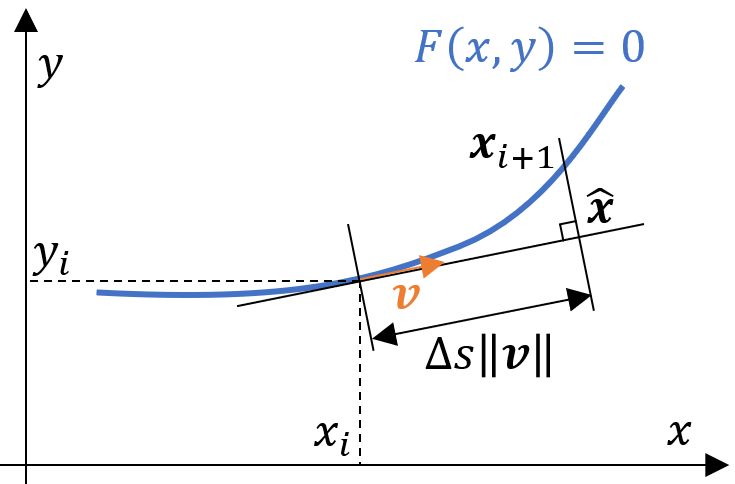
\includegraphics[width=.62\linewidth,trim={0.000bp 0.000bp 0.500bp 1.500bp},clip]{graphics/pszeudo_ivhossz_szemleltet.png}
	\caption{A pseudo-arclength continuation eljárás egy iterációs lépésének szemléltetése}\label{fig:pszeudo_ivhossz_szemleltet}
\end{figure}

A módszer alkalmazása során a \eqref{eq:pszeudo_ivhossz_alapegyenlet} egyenletrendszert szimultán kell megoldani $\mathbf{x}_{i+1}$-re - két egyenlet, két ismeretlen.
A módszer általánosítható több dimenzióra is, ekkor több $F_j(\mathbf{x})$ egyenletre van szük\-sé\-günk.

\exampleheading{Példa: körív követése.}
Akkor az implicit függvényünk az alábbi:
\begin{equation}
F(\mathbf{x}) = x^2 + y^2 -1.
\end{equation}
A kezdőpontunk legyen
\begin{equation}
\mathbf{x}_0 = \begin{bmatrix}
1 & 0
\end{bmatrix}^\mathrm{T},
\end{equation}
amely, mint látható kielégíti az implicit egyenletünket.
A sebességvektor, azaz az érintő ebben a pontban
\begin{equation}
\mathbf{v}_0 = \begin{bmatrix}
0 & 1
\end{bmatrix}^\mathrm{T}.
\end{equation}
Azonban az esetek többségében ez nem ilyen egyszerűen meghatározható, és numerikusan kell közelítenünk, amihez ismernünk kell a szintvonal egy másik, közeli pontját is, $\mathbf{x}_{1/2}$-et:
\begin{equation}
\mathbf{v}_0 = \frac{\mathbf{x}_{1/2} - \mathbf{x}_{0}}{\left \| \mathbf{x}_{1/2} - \mathbf{x}_{0} \right \|}.
\end{equation}
A sebességvektor ezek után rendre:
\begin{equation}
\mathbf{v}_i = \frac{\mathbf{x}_{i} - \mathbf{x}_{i-1}}{\left \| \mathbf{x}_{i} - \mathbf{x}_{i-1} \right \|}.
\end{equation}
A körív követésének eredménye a pseudo-arclength continuation eljárással a \ref{fig:pszeudo_ivhossz_koriv}. ábrán látható.
A lépéshossz $\Delta s = 0.1$ volt, a kezdeti sebességbecsléshez az $\mathbf{x}_0$-hoz közeli szintvonal pont pedig
\begin{equation}
\mathbf{x}_{1/2} = \begin{bmatrix}
0.99 & \sqrt{1 - 0.99^2}
\end{bmatrix}^\mathrm{T}.
\end{equation}

\begin{figure}[ht]
	\centering
	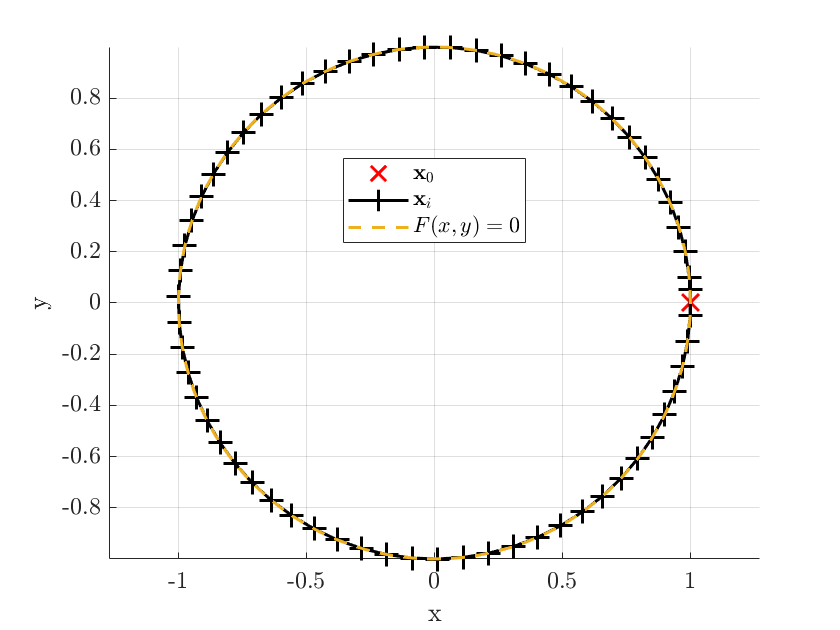
\includegraphics[width=\linewidth,trim={22.497bp 3.000bp 56.243bp 22.497bp},clip]{graphics/pszeudo_ivhossz_koriv.png}
	\caption{A pseudo-arclength continuation eljárás alkalmazása körív követésére}\label{fig:pszeudo_ivhossz_koriv}
\end{figure}
\exampleend

\paragraph*{Érintő, skálázás és lépésvezérlés.}
Az érintő közvetlenül is számítható $DF(\mathbf x_i)\mathbf v_i=0$, $\|\mathbf v_i\|=1$ alapján; orientációját az előző érintővel pozitív skalárszorzat rögzíti. A szekánsirány olcsó közelítés. Különböző mértékegységű változóknál először skálázni kell a koordinátákat, vagy súlyozott skalárszorzatot használni. Sikertelen Newton-korrekciónál csökkentjük a lépéshosszt. A korrekció során a korábbi megoldás és az érintő változatlan; csak elfogadott lépés után frissítjük őket.

A melléklet \texttt{pal\_corrector\_v3.m} függvénye az egész kibővített egyenletrendszert oldja meg, egy érintőkomponenssel sem oszt. Körön például $G(y)=y_1^2+y_2^2-1$ használható. Az általános $G:\mathbb R^q\to\mathbb R^{q-1}$ reziduum lehet egy diszkretizált peremfeladat is.

\FloatBarrier
\exampleheading{Példa: áthaladás egy visszahajláson.}
A $\dot x=\mu-x^2$ rendszer egyensúlyai $G(x,\mu)=\mu-x^2=0$ görbét alkotnak. $\mu>0$ mellett az $x=+\sqrt\mu$ ág stabil, az $x=-\sqrt\mu$ ág instabil; $\mu=0$-nál találkoznak. A $\mu$ szerinti egyirányú léptetés itt megakad, míg a pseudo-arclength continuation eljárás átjut az $x=0$ ponton. A függelékben közölt rövid program közvetlenül a melléklet korrektorát használja, globális változók nélkül. A két kezdőpont ismert egyensúly; minden új pontot a két előzőből számítunk.
\phantomsection\label{use:fold}A teljes MATLAB-program az A függelék \ref{ap:fold}. szakaszában található (\pageref{ap:fold}. oldal).
\exampleend

\section{Közönséges differenciálegyenletek peremérték-feladatai}

A \emph{peremérték-feladat} (angolul: \emph{Boundary Value Problem}, röviden BVP) olyan közönséges differenciálegyenlet vagy egyenletrendszer megoldását keresi, amelyre a keresett függvény az integrálási tartomány \emph{mindkét végpontjában} megadott feltételeknek kell, hogy eleget tegyen.

Legyen adott egy $n$-edrendű közönséges differenciálegyenlet az ismeretlen $y(x)$ függvényre:
\[
F\big(x, y, y', y'', \ldots, y^{(n)}\big) = 0,
\qquad x \in [a,b].
\]
Szeparált peremfeltételek az alábbi alakban adhatók meg; a periodikus feltételek a két végpontot közvetlenül összekapcsolják:
\[
B_a\big(y(a), y'(a), \ldots, y^{(n-1)}(a)\big) = 0,
\qquad
B_b\big(y(b), y'(b), \ldots, y^{(n-1)}(b)\big) = 0,
\]
ahol $B_a$ és $B_b$ a bal és jobb határpontban előírt feltételeket jelölik.

\begin{itemize}
\item A \emph{kezdeti érték feladat} (IVP) esetén a megoldás és annak származtatott értékei egyetlen pontban (általában $x=a$-ban) ismertek. Amennyiben a feladat korrekt kitűzésű, a megoldás létezése és egyértelműsége biztosított.
\item A \emph{peremérték-feladat} ezzel szemben olyan feladat, ahol az előírt feltételek különböző pontokban (pl. $x=a$ és $x=b$) adottak. A BVP tehát tipikusan „kétponti” feltételrendszert jelent, de többpontos általánosítás is lehetséges. Egy BVP-nek lehet nulla, egyetlen, több véges számú vagy végtelen sok megoldása.
\end{itemize}

\subsection{Megoldási módszerek}

A peremérték-feladatok többsége nem oldható meg analitikusan, ezért numerikus módszereket alkalmazunk. A leggyakrabban használt eljárások:

\begin{itemize}
  \item \textbf{Shooting módszer:}
  A BVP-t kezdeti érték feladattá alakítja úgy, hogy az ismeretlen kezdeti feltételeket iteratív módon módosítja, amíg a jobb oldali peremfeltétel teljesül.

  \item \textbf{Multiple shooting módszer:}
  A tartományt több szakaszra osztja, és minden szakaszon külön IVP-t old meg, majd a megoldásokat illeszti össze a csatlakozási feltételek alapján.

  \item \textbf{Kollokációs módszerek:}
  A keresett megoldást közelítő függvények (pl. polinomok, spline-ok) lineáris kombinációjaként írják fel, és az egyenletet diszkrét pontokban kényszerítik teljesülni.

  \item \textbf{Véges differencia (finite difference) módszer:}
  Az egyenletet differenciaközelítésekkel diszkretizálja, így egy algebrai egyenletrendszert kapunk a rácspontokban definiált $y_i$ értékekre.
\end{itemize}

\subsection{Példa: függőleges feldobás előírt csúcsmagassággal}
\examplebody

Egy testet függőlegesen feldobunk, légellenállás nélkül. Mekkora kezdeti sebesség szükséges ahhoz, hogy pontosan $h=1\,\mathrm m$ magasságban álljon meg egy pillanatra? A kezdeti sebesség és a csúcs elérésének $T$ ideje is ismeretlen. Ez a kétdimenziós lövedékmozgásnál egyszerűbb példa ugyanazt a gondolatot mutatja: a hiányzó kezdeti adatot végponti feltételekből számítjuk ki.
\begin{equation}
\dot y=v,\qquad \dot v=-g,\qquad y(0)=0,\quad y(T)=h,\quad v(T)=0.
\end{equation}
A $\tau=t/T\in[0,1]$ transzformációval
\begin{equation}
\frac{d}{d\tau}\begin{pmatrix}y\\v\end{pmatrix}
=T\begin{pmatrix}v\\-g\end{pmatrix}.
\end{equation}
Két állapothoz és egy szabad időparaméterhez három peremfeltétel tartozik. A pozitív időtartamú megoldást keressük. Ellenőrzésként
\[
T=\sqrt{2h/g}\simeq0{,}451524\,\mathrm s,\qquad
v(0)=\sqrt{2gh}\simeq4{,}429447\,\mathrm{m/s}.
\]
A teljes programban a differenciálegyenletet, a peremfeltételeket és a kezdeti becslést rövid anonim függvények adják meg; nincs külön segédfájl.
\phantomsection\label{use:apex_bvp}A teljes MATLAB-program az A függelék \ref{ap:apex_bvp}. szakaszában található (\pageref{ap:apex_bvp}. oldal).

Ugyanezt a feladatot shooting módszerrel is megoldjuk: egy próbált $v_0$ sebességgel a $v=0$ eseményig integrálunk, majd a csúcsmagasság hibáját nullázzuk. A $[1,8]\,\mathrm{m/s}$ intervallum közrefogja a megoldást; a választott $2\,\mathrm s$ integrálási idő minden itt próbált sebességnél elegendő a csúcs eléréséhez. Így a két módszer ugyanazon analitikusan ellenőrizhető feladaton hasonlítható össze.
\phantomsection\label{use:apex_shooting}A teljes MATLAB-program az A függelék \ref{ap:apex_shooting}. szakaszában található (\pageref{ap:apex_shooting}. oldal).
\exampleend

\section{Periodikus pályák peremérték-megfogalmazása}
\label{sec:per_palya_perem_megfog}

Dinamikai rendszerek mozgásegyenleteinek megoldásakor kezdeti értéket szoktunk megadni.
Amennyiben a rendszer periodikus mozgást végez, a probléma átírható egy peremérték feladatra, ahol a peremfeltételt a periódus elejére és végére kell előírni.
Belátható ugyanis, hogy periodikus mozgásnál az állapotváltozóknak $t_0$ és $t_0 + T$ időpontokban meg kell egyezniük, ahol $T$ a periódusidő.
Dinamikai rendszerek mozgásegyenleteit Cauchy átírással általánosan az alábbi módon lehet megadni:
\begin{equation}
\dot{\mathbf{z}}(t) = \mathbf{F}(\mathbf{z}(t)),
\label{eq:EOM_altalanosan}
\end{equation}
ahol $\mathbf{z}(t)$ az állapotváltozók, $\mathbf{q}(t)$ pedig az általános koordináták vektora:
\begin{equation}
\mathbf{z}(t) = \begin{bmatrix}
\mathbf{q}(t) & \dot{\mathbf{q}}(t)
\end{bmatrix}^\mathrm{T}.
\end{equation}
Periodikus mozgás esetén (autonóm rendszereknél $t_0$ szabadon megválasztható, így vegyük zérusnak) igaz a következő
\begin{equation}
\mathbf{z}_\mathrm{p}(0) = \mathbf{z}_\mathrm{p}(T) .
\end{equation}

Vezessük be $\tau$ dimenziótlan időt az alábbi módon:
\begin{equation}
\tau =  t/T.
\end{equation}
Ekkor a \eqref{eq:EOM_altalanosan} egyenlet formája és a peremérték feladat a következő lesz
\begin{equation}
\begin{cases}
\mathbf{z}'(\tau) = T\,\mathbf{F}(\mathbf{z}(\tau)), \\
\mathbf{z}(0) = \mathbf{z}(1).
\end{cases}
\label{eq:EOM_dimtalan}
\end{equation}

Láthatjuk, hogy az egyenletek száma megegyezik a peremfeltételek számával, ám egy ismeretlen paraméter $T$ is része a feladatnak. Így még egy peremfeltétel szükséges. Intuitív módon erre azért van szükség, mert a $\mathbf{z}(0) = \mathbf{z}(1)$ feltétel nem rögzíti a megoldás kezdetét (fázisát), így a fenti feladatnak végtelen sok megoldása van.

A hiányzó egyenlet az ún. fázisfeltétel, amely "kiválasztja" azt az egyetlen megoldást, amellyel a feladat korrekt kitűzésű lesz. Számos lehetőség van, itt tekintsük azt az esetet, amikor egy paraméter változtatása mellett követjük a periodikus pályát; egy korábbi $\mu$ paraméterérték esetén már rendelkezésre áll egy pálya, amely $t=0$-ban az $z_p(0)$ értéket veszi fel (a $p$ index a previous-ra utal). Keressük a periodikus pályát $\mu+ \Delta \mu$ paraméterérték esetében. A fázisfeltétel:

\begin{equation}
0=\left< \mathbf{z}_p(0)-\mathbf{z}(0),\mathbf{F}(\mathbf{z}_p(0))\right>,
\end{equation}

\noindent ami azt jelenti, hogy a régi és új (ismeretlen) pályák $t=0$-t összekötő vektora merőleges legyen a (régi) pálya érintőjére.

Amennyiben a rendszerünk szakaszosan folytonos, a \eqref{eq:EOM_dimtalan}-es problémát ki kell egészíteni azzal, hogy megfelelő időpontokban a pályának a kapcsolóvonalon kell elhelyezkednie.

\begin{equation}
\begin{matrix}
\begin{cases}
\mathbf{z}'(\tau_1) = T_1\,\mathbf{F}_1(\mathbf{z}(\tau_1)), \; H(\mathbf{z}(\tau_1)) > 0,\\
\mathbf{z}'(\tau_2) = T_2\,\mathbf{F}_2(\mathbf{z}(\tau_2)), \; H(\mathbf{z}(\tau_2)) < 0,
\end{cases} \\[4pt]
\begin{cases}
\mathbf{z}_1(1) = \mathbf{z}_2(0), \\
\mathbf{z}_2(1) = \mathbf{z}_1(0),
\end{cases} \\[4pt]
\begin{cases}
H(\mathbf{z}_1(1)) = 0, \\
H(\mathbf{z}_2(1)) = 0,
\end{cases}
\end{matrix}
\end{equation}
ahol $H(\mathbf{z}(\tau))$  a kapcsolófelület.
Ütköző rendszer esetében figyelembe kell venni a peremfeltételek felírásánál az ütközéskor létrejövő leképezést.

Nézzük meg egy egyszerű példát! A mechanikai rendszerünk a \ref{fig:bvp_tomeg_rugo}. ábrán látható.

\begin{figure}[ht]
	\centering
	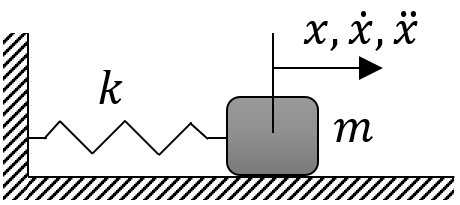
\includegraphics[width=.45\linewidth,trim={0.000bp 0.000bp 0.000bp 3.000bp},clip]{graphics/tomeg_rugo_modell.png}
	\caption{Periodikus mozgást végző tömeg-rugó rendszer}\label{fig:bvp_tomeg_rugo}
\end{figure}

A mozgásegyenlete a fenti rendszernek jól ismert:
\begin{equation}
\ddot{x}= -\frac{k}{m}\,x.
\end{equation}
Mint tudjuk, a rendszer mozgását leíró függvényt az alábbi módon lehet felírni, amennyiben $x_0$ kezdeti kitérítésünk van csak $\tau_0$ időpillanatban kezdeti sebesség nélkül:
\begin{equation}
\varphi(\tau) = x_0\cos\left(\tau\sqrt{k/m}\,T\right) = x_0\cos\left(2\pi\,\tau\right),
\end{equation}
\begin{equation}
\dot{\varphi}(\tau) = -x_0\sqrt{k/m}\sin\left(\tau\sqrt{k/m}\,T\right) = -x_0\sqrt{k/m}\sin\left(2\pi\,\tau\right),
\end{equation}
ahol $T$ a rendszer sajátfrekvenciájának inverze
\begin{equation}
T = 2\pi\sqrt{m/k}.
\end{equation}
A fenti függvényeket a peremérték-megfogalmazáskor kijöttekkel fogjuk összevetni.

A bvp5c megoldóhoz először definiálnunk kell egy időrácsot, amely i\-dő\-pon\-tok\-ban meg kell becsülnünk majd a keresett függvények értékét.
Mivel áttértünk dimenziótlan időre, egy periódus "peremei" a $\tau \in \left \{ 0,1 \right \}$ pontok, valamint megjelent a Cauchy átírásnál $T$ periódusidő, mint ismeretlen paraméter.
\begin{equation}
\begin{bmatrix}
x'(\tau) \\ y'(\tau)
\end{bmatrix} =
T
\begin{bmatrix}
y(\tau) \\  -\frac{k}{m}\,x(\tau)
\end{bmatrix}
\end{equation}
A harmonikus oszcillátor konzervatív: a periodikus pályák amplitúdó szerint családot alkotnak. Ezért az általános periodicitási és fázisfeltétel mellett az amplitúdót is rögzíteni kell. Az $x(0)=x_0$, $x(1)=x_0$, $v(0)=0$ három feltétel használata sem megfelelő: a periódus végén $v(T)=0$, így a véghelyzet periódusidő szerinti deriváltja nulla, és a linearizált peremfeladat szinguláris.

Ebben a szimmetrikus példában egyszerűbb egy \emph{negyed periódust} számítani. Legyen $Q=T/4$ és $\theta=t/Q\in[0,1]$. A megoldandó feladat:
\[
\frac{d}{d\theta}\begin{pmatrix}x\\v\end{pmatrix}
=Q\begin{pmatrix}v\\-(k/m)x\end{pmatrix},\qquad
x(0)=x_0>0,\quad v(0)=0,\quad x(1)=0.
\]
Két differenciálegyenlethez és az egyetlen ismeretlen $Q$ paraméterhez három peremfeltétel tartozik. Az első zérushelyet keressük, $v(1)<0$ mellett, ezért $\partial_Q x(Q)=v(Q)\neq0$. A megfelelő kezdeti becslés az első negyed periódushoz választja ki a megoldást; ezt a kód az $x>0$ belső feltétellel is ellenőrzi. A teljes periódus $T=4Q$. Ez a szimmetriára épülő konstrukció a harmonikus példára vonatkozik, általános határciklusnál a korábban bemutatott periodicitási és fázisfeltételt kell használni.

A függelékben megadott teljes programot \texttt{mass\_spring\_bvp\_v3.m} néven mentsük el, majd a MATLAB aktuális könyvtárából a \lstinline|[T,sol] = mass_spring_bvp_v3;| paranccsal indítsuk. Az alapértékek $k=10$, $m=5$, $x_0=1$; más értékek például a \lstinline|mass_spring_bvp_v3(10,5,1)| hívással adhatók meg. A differenciálegyenletet és a peremfeltételeket leíró függvények ugyanebben a fájlban szerepelnek, külön segédfájl nem szükséges.
\phantomsection\label{use:spring_bvp}A teljes MATLAB-program az A függelék \ref{ap:spring_bvp}. szakaszában található (\pageref{ap:spring_bvp}. oldal).

A kód kiírja a $T=4Q$ eredményt és a $2\pi\sqrt{m/k}$ analitikus periódust, az ábrán pedig összehasonlítja a numerikus és az analitikus megoldást. A kód a négy negyedperiódust a numerikus megoldás tükrözésével és előjelváltásaival állítja össze. A kék görbe az analitikus megoldás, a narancssárga körök a peremfeladatból származó értékek. Az elmozdulás és a sebesség külön panelen látható, saját mértékegységgel. Az ábra 16 cm széles, feliratai 11 pontosak; a PDF-et átméretezés nélkül illesztjük be. A program a vektoros PDF- és SVG-fájlt is elmenti.
A teljes periódusra folytatott pozíciót és sebességet a \ref{fig:bvp_tomeg_rugo_traj_vel}. ábra szemlélteti.

\begin{figure}[ht]
	\centering
	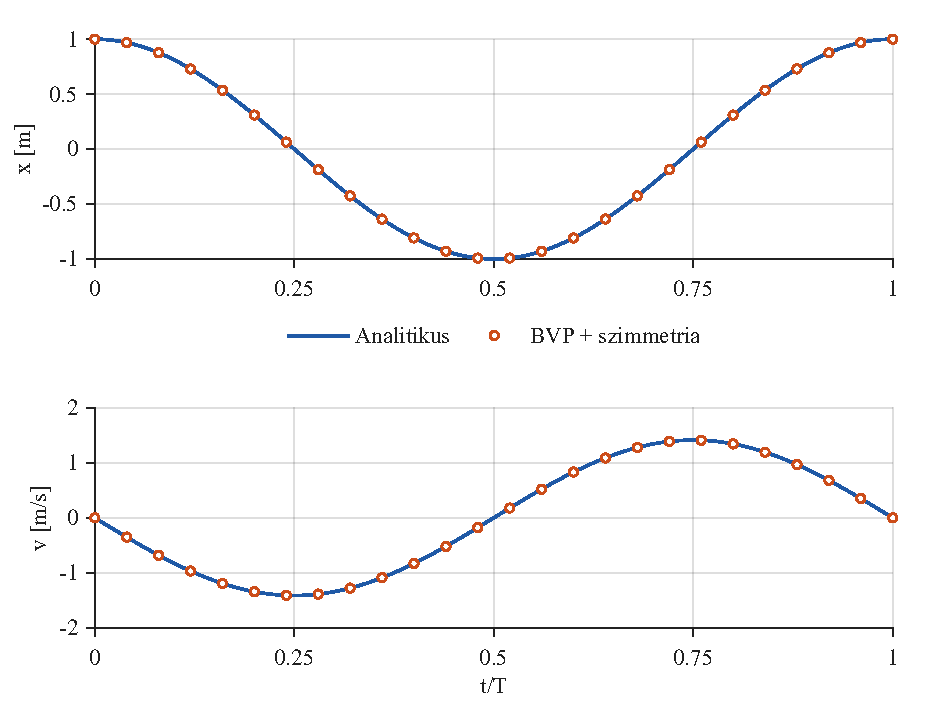
\includegraphics{graphics_v3/mass_spring_bvp.pdf}
	\caption{Tömeg--rugó rendszer teljes periódusa: fent az elmozdulás, lent a sebesség, $k=10$ N/m, $m=5$ kg, $x_0=1$ m mellett. A \texttt{bvp5c} negyedperiódus-megoldását szimmetriával folytatjuk; a körök és az analitikus görbe gyakorlatilag fedik egymást.}\label{fig:bvp_tomeg_rugo_traj_vel}
\end{figure}

\section{A teljes periodikus peremfeladat folytatása}
\label{sec:full_pal}
A $T=T_{\mathrm{BVP}}(\mu)$ grafikon feltevése egyszerű példákban használható, de általános visszahajlásnál a pálya nem egyértékű függvénye $\mu$-nek. Ilyenkor a teljes $y=(z(\cdot),T,\mu)$ megoldás az ismeretlen. Egy autonóm, sima rendszerre a korrekció egyidejűleg oldja meg
\begin{align}
z'(\tau)&=T F(z(\tau),\mu),\qquad z(0)=z(1),\\
0&=\int_0^1\langle z(\tau)-z_i(\tau),z_i'(\tau)\rangle\,d\tau,\\
\Delta s&=\int_0^1\langle z(\tau)-z_i(\tau),v_z(\tau)\rangle_W\,d\tau\notag\\
&\quad+w_T(T-T_i)v_T+w_\mu(\mu-\mu_i)v_\mu.
\end{align}
A második sor fázisfeltétel, a harmadik a pseudo-arclength feltétele; a súlyok és a normalizált érintő ugyanahhoz a skálázáshoz tartoznak. Konzervatív pályacsaládnál további energiarögzítés és szükség esetén megfelelő kibővítés kell, ahogy a harmonikus példánál is láttuk. Több folytonos szegmens esetén a teljes diszkretizált rendszer a szegmenseket, a kapcsolási vagy reset feltételeket és az ismeretlen szegmensidőket is tartalmazza. Ez a felírás nem oszt egy érintőkomponenssel, és egyszerű fordulóponton is használható \cite{auto}.

\section{Pseudo-arclength continuation periodikus pályákra}

Ebben az alfejezetben két egyszerű periodikus pályacsaládot vizsgálunk. Megkülönböztetjük a rögzített paraméterű peremfeladat megoldását, a közvetlen paraméterléptetést és a visszahajláshoz szükséges pseudo-arclength continuation eljárást.
Ehhez ki kell választanunk majd egy bifurkációs paramétert, amely függvényében kíváncsiak vagyunk, hogyan alakul a periodikus mozgás.
Az első feladat az előbb vizsgált tömeg-rugó rendszer paraméterfüggését mutatja be; a másodikban a merevség a kitérés előjelével vált, ezért két folytonos szegmenst illesztünk össze.

\subsection{Példa 1: tömeg-rugó rendszer}
\examplebody


A pseudo-arclength continuation eljárás használatához ki kell választanunk egy bi\-fur\-ká\-ci\-ós paramétert, amit jelöljön $\mu$.
A példa során először vizsgáljuk a rugómerevség $(\mu = k)$, később a tömeg $(\mu =m)$ hatását (ilyenkor a többi paraméter konstans).
A \eqref{eq:pszeudo_ivhossz_alapegyenlet} egyenlet alakja paraméterkövetés során az alábbi formájú:
\begin{equation}
\begin{cases}
0 = \left< \mathbf{x}_{i+1} - \mathbf{x}_i, \mathbf{v}_i \right> - \Delta s \\
0 = T_{i+1} - T_{\mathrm{BVP}}(\mu_{i+1}),
\end{cases}
\label{eq:pszeudo_per_kov}
\end{equation}
\begin{equation}
\mathbf{x_i}= \begin{bmatrix}
\mu_{i} & T_{i}
\end{bmatrix}^\mathrm{T},
\end{equation}
ahol $T_{\mathrm{BVP}}(\mu_{i+1})$ a peremfeladat-megoldó által számolt periódusidő. Ez a csökkentett felírás itt megengedett, mert $k,m>0$ mellett $T=2\pi\sqrt{m/k}$ sima, egyértékű grafikon. Általános pályacsaládra a \ref{sec:full_pal}. szakasz teljes feladatát kell használni.
A pseudo-arclength continuation eljárást a \ref{sec:pseudo_ivhossz} alfejezetben bemutatott módon kell alkalmazni, és a benne található $T_{\mathrm{BVP}}(\mu_{i+1})$ értékét a \ref{sec:per_palya_perem_megfog} alfejezetben leírt módon kell meghatározni a \eqref{eq:pszeudo_per_kov} egyenletrendszer megoldása közben.
A kapott eredményeket összevetettük az analitikusan kiszámítottakkal, és látható, hogy a pályakövetés illeszkedik az analitikusan előállított görbékre, ld. \ref{fig:pszeudo_tomeg_rugo_k}. és \ref{fig:pszeudo_tomeg_rugo_m}. ábrák.

A fájl neve: \texttt{spring\_continuation\_v3.m}. Indítás MATLAB-ban: \lstinline|spring_continuation_v3|. Minden periódust a \texttt{bvp5c} számít, az analitikus képlet csak a kezdeti becsléshez és az eredmény ellenőrzéséhez szerepel. A szelőirányú prediktort kétdimenziós Newton-korrektor követi: a periódus maradéka mellett a prediktorra merőleges hipersík feltételét oldjuk meg. A periódus paraméterderiváltját középpontos differenciával becsüljük. A korrektor így nem igényel \texttt{fsolve}-ot vagy külön segédfájlt.

A merevségkövetés $k=2$ N/m-ről indul, $m=5$ kg és $\Delta s=0{,}5$ mellett; a tömegkövetés $m=1$ kg-ról indul, $k=10$ N/m és $\Delta s=1$ mellett. Mindkét esetben két kezdőpont után 30 korrekciós lépést végzünk. A lépéshosszt itt a megadott egységekben felírt $(\mu,T)$ koordináták euklideszi normájával mérjük; más egységek vagy léptékek esetén skálázás szükséges. Az analitikus görbe és a numerikus körjelölők egyezése a peremfeladatot és a követést ellenőrzi; ezen a monoton ágon nincs visszahajlás.
\phantomsection\label{use:spring_cont}A teljes MATLAB-program az A függelék \ref{ap:spring_cont}. szakaszában található (\pageref{ap:spring_cont}. oldal).

\begin{figure}[!htbp]
	\centering
	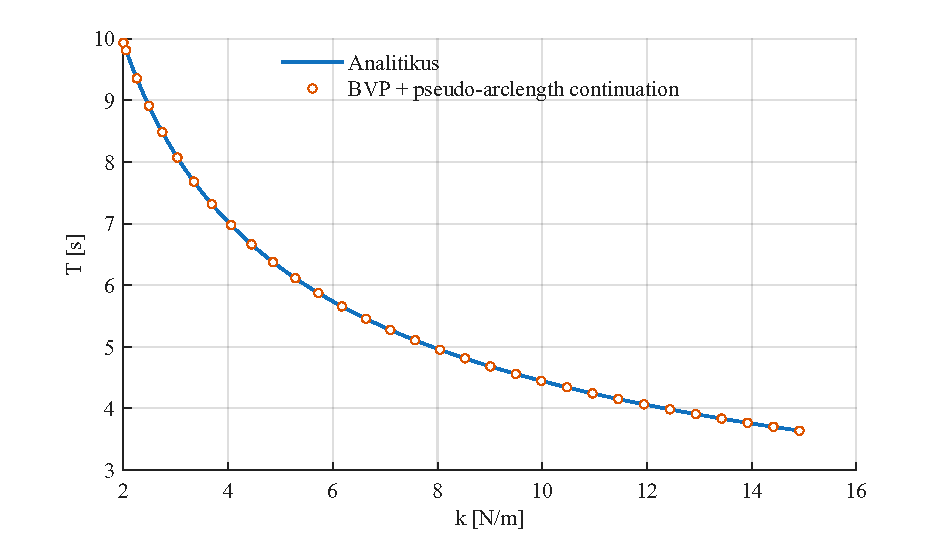
\includegraphics{graphics_v3/spring_k.pdf}
	\caption{Periodikus pályák követése $k$ paraméter függvényében, $\Delta s = 0.5$}\label{fig:pszeudo_tomeg_rugo_k}
\end{figure}

\begin{figure}[!htbp]
	\centering
	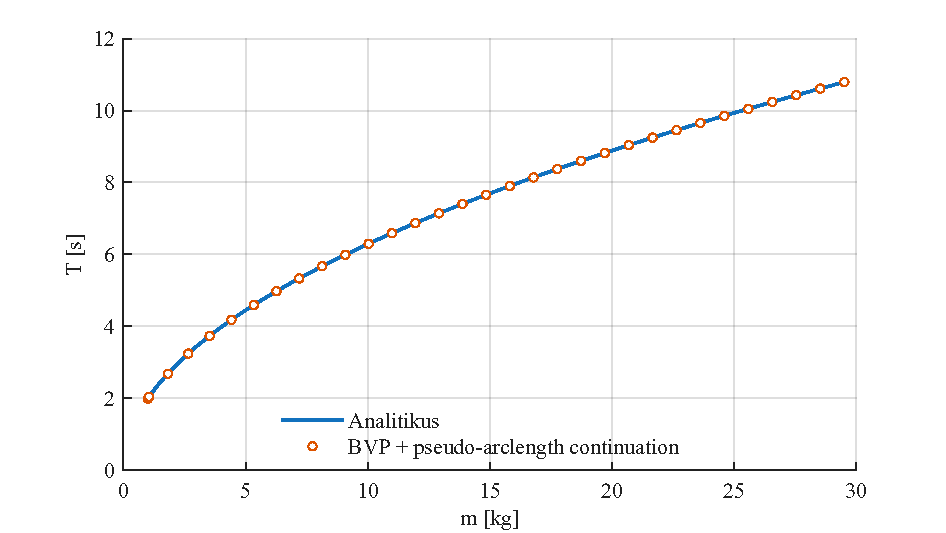
\includegraphics{graphics_v3/spring_m.pdf}
	\caption{Periodikus pályák követése $m$ paraméter függvényében, $\Delta s = 1$}\label{fig:pszeudo_tomeg_rugo_m}
\end{figure}

\FloatBarrier
\exampleend

\subsection{Példa 2: kétféle merevségű rugó}
\examplebody

A több szegmensből összeállított peremfeladatot egy egységnyi tömegű, kétféle rugómerevségű oszcillátoron mutatjuk be:
\begin{equation}\label{eq:bilinear_oscillator}
\ddot x=\begin{cases}-k_+x,&x>0,\\-k_-x,&x<0,\end{cases}
\qquad k_+,k_->0.
\end{equation}
A kapcsolófelület $x=0$. Az állapot folytonos, nincs sebességugrás. A vektormező itt folytonos, csak a deriváltja vált: ez a piecewise-smooth rendszerek legegyszerűbb esete. A kapcsolófelületen a saltation-mátrix az identitás, ezért ez a példa a szegmensek illesztését tanítja; a nemtriviális ütközési korrekciót az ütköző oszcillátor mutatja be.

Induljunk $x(0)=0$, $v(0)=V>0$ állapotból. A pozitív és negatív félhullámot külön $[0,1]$ időskálára írjuk át, ismeretlen $T_+$ és $T_-$ időkkel. A négy komponens $(x_+,v_+,x_-,v_-)$, a hat peremfeltétel pedig
\begin{align}
x_+(0)&=0,&v_+(0)&=V,&x_+(1)&=0,\\
x_-(0)&=x_+(1),&v_-(0)&=v_+(1),&x_-(1)&=0.
\end{align}
Az első feltétel a fázist, a második az energiaszintet rögzíti. A végső sebesség $v_-(1)=V$ az energiamegmaradásból és az első félhullámok kiválasztásából következik; külön előírva túlhatároznánk ezt a hatfeltételes feladatot. Az analitikus ellenőrzés:
\begin{equation}
T_+=\frac{\pi}{\sqrt{k_+}},\qquad
T_-=\frac{\pi}{\sqrt{k_-}},\qquad T=T_++T_-.
\end{equation}
A $k_+=4$, $k_-=1$, $V=1$ választásnál $T=3\pi/2$. A kód négy állapotot és két ismeretlen időt kezel, és megköveteli a megfelelő félhullámok előjelét. Az analitikus alak csak kezdeti becslés és ellenőrzés; az időtartamokat a peremfeladat-megoldó számítja.
A teljes, önálló programot \texttt{bilinear\_bvp\_v3.m} néven mentve a \lstinline|[T,sol] = bilinear_bvp_v3;| paranccsal indíthatjuk. A két lokális függvény ugyanebben a fájlban szerepel. A program a félhullámok illesztésén túl a teljes periódust ábrázolja, és vektoros PDF- és SVG-fájlt ment. A feliratok 11 pontosak; az ábrát átméretezés nélkül illesztjük be.
\phantomsection\label{use:bilinear}A teljes MATLAB-program az A függelék \ref{ap:bilinear}. szakaszában található (\pageref{ap:bilinear}. oldal).

\begin{figure}[htbp]
\centering
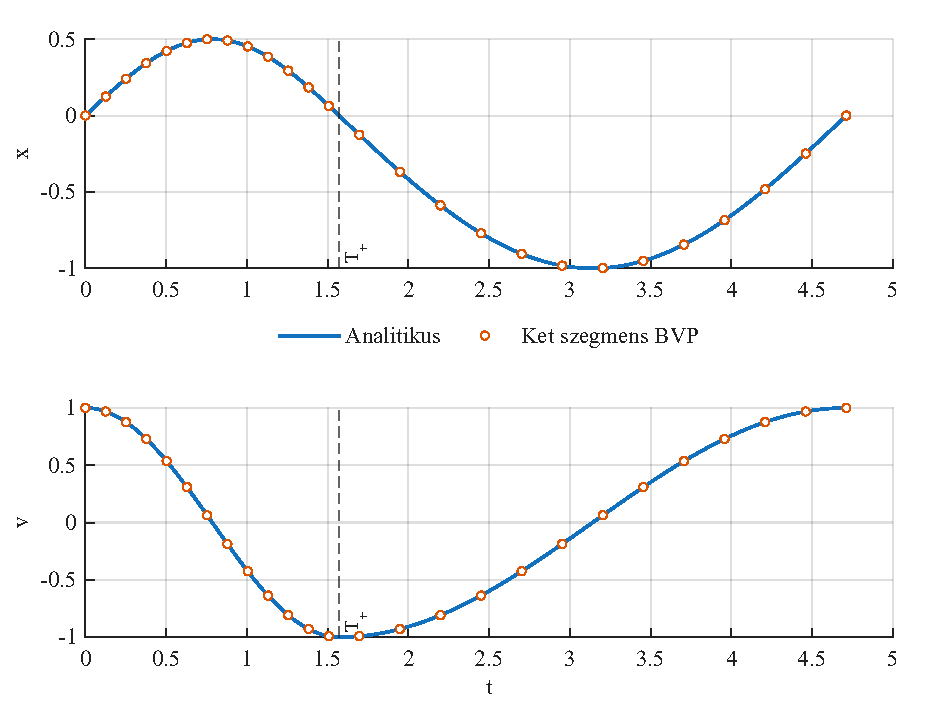
\includegraphics{graphics_v3/bilinear_bvp.pdf}
\caption{A kétféle merevségű oszcillátor egy teljes periódusa, $k_+=4$, $k_-=1$, $V=1$ mellett. Fent az elmozdulás, lent a sebesség; folytonos vonal: analitikus megoldás, körök: a két szegmensből illesztett BVP-megoldás. A szaggatott vonal $T_+=\pi/2$ időpontját jelöli.}\label{fig:bilinear_bvp}
\end{figure}

A \ref{fig:bilinear_bvp}. ábrán a merevebb, pozitív oldali félhullám rövidebb ($T_+=\pi/2$), és kisebb a kitérése ($x_{\max}=1/2$). A lágyabb, negatív oldalon $T_-=\pi$ és $x_{\min}=-1$. Az illesztéskor $x=0$ és $v=-1$ mindkét szegmensben ugyanaz: nincs állapotugrás. A periódus végén $(x,v)=(0,1)$, tehát a pálya záródik. A pontok és az analitikus görbék egyezése külön-külön ellenőrzi a két szegmenst és az illesztésüket.


Ez rögzített paraméterű többfázisú BVP, önmagában nem pseudo-arclength continuation. Itt $k_+$ szerinti közvetlen paraméterléptetés is elegendő: $T(k_+)=\pi/\sqrt{k_+}+\pi/\sqrt{k_-}$ nem hajlik vissza. Általános visszahajlásnál a \ref{sec:full_pal}. szakasz teljes kibővített rendszerét kell használni. A korábbi, összetettebb SLIP-peremfeladat kódja további alkalmazásként a \texttt{codes/slip\_bvp\_v3.m} fájlban elérhető; nem szükséges a két szegmens illesztésének megértéséhez.
\exampleend

\section{Stabilitási és grazing-határok követése}
Egy bifurkációs görbe követéséhez két \emph{fizikai} paramétert választunk, például az ütköző oszcillátor gerjesztési frekvenciáját és falhelyzetét, $(\mu_1,\mu_2)=(\omega,\sigma)$. A teljes periodikus peremfeladatot egy skalár kritikus feltétellel, majd a pseudo-arclength egyenlettel egészítjük ki. A $\lambda$ multiplikátor nem új, szabad fizikai paraméter: a pálya monodrómia-mátrixából kell számítani vagy sajátvektor-egyenlettel csatolni.

Példák: nemtriviális $\lambda=+1$ ciklusok saddle-node bifurcation eseményének jelöltje, $\lambda=-1$ period-doubling bifurcation jelöltje, nemvalós $|\lambda|=1$ pár Neimark--Sacker-bifurkáció jelöltje. Az autonóm időeltolás és a konzervált energia triviális egységnyi multiplikátorait előbb ki kell szűrni, például megfelelő Poincaré-metszettel és energiaszintre megszorítással. A kritikus feltétel önmagában nem garantál nemelfajult bifurkációt.

Grazing-határnál az eseménypont a kapcsolófelületen van és $H_xF=0$; a reguláris esethez $a_H\neq0$ is kell. A transzverzális saltation-mátrixot a grazing-pontban nem szabad véges numerikus értékként használni.
